%! TEX program = xelatex
% WARNING: this is a generated file.
%
% Please do not edit this file directly. 
% - If you want to update the medatata of the paper (title, authors, abstract), please
%   edit the `paper-meta.yaml` file in the root of the repository.
% - If you want to update the content of the paper, please edit the latex files
%   in the `src` directory.
% - If you want to update the template itself (e.g., change the layout), please
%   edit the `templates/lipics/lipics.tex` file instead.
\documentclass[
    a4paper,
    UKenglish,
    cleveref,
    autoref,
    thm-restate]{lipics-v2021}

\usepackage{todonotes}
\usepackage{lineno}
\linenumbers




% math packages
\usepackage{stmaryrd,thmtools,upgreek}
\usepackage{amsmath,amssymb,amsfonts}

% graphics packages
\usepackage{graphicx}
\usepackage[obeyclassoptions,mode=tex]{standalone}
\usepackage{tikz}
\usetikzlibrary{backgrounds}
\usetikzlibrary{calc}
\usetikzlibrary{shapes.geometric}
\usetikzlibrary{positioning}
\usetikzlibrary{automata}
\usetikzlibrary{tikzmark}
\usetikzlibrary{patterns}
\usetikzlibrary{arrows}
\tikzset{every state/.style={minimum size=1pt}}
\usepackage{tikz-cd}


% links inside the document
\usepackage[composition,hyperref,xcolor,cleveref]{knowledge}
\knowledgeconfigure{notion}

% Tables 
\usepackage{booktabs}
\usepackage{varwidth}

% Packages for macro definitions
\usepackage{xparse}
\usepackage{xpatch}
\usepackage{tokcycle}
\usepackage{ifthen}

% Proofs
\usepackage{bussproofs}

% Colors 
\usepackage{ensps-colorscheme}


% we include whatever the user wants to include in the header

% we include libraries (tex files) usually written in the `lib` directory
% Upgreek letters
\makeatletter
\newcommand\mathgr[1]{\tokcycle
  {\addcytoks{##1}}
  {\processtoks{##1}}
  {\ifcsname up\expandafter\@gobble\string##1\endcsname
   \addcytoks[1]{\csname up\expandafter\@gobble\string##1\endcsname}%
    \else\addcytoks{##1}\fi}
  {\addcytoks{##1}}{#1}%
  \expandafter\mathrm\expandafter{\the\cytoks}%
}
\makeatother



% Create a new macro proofof
% taking as input a label of a theorem
% and creating a proof with a reference to that
% label
\NewDocumentEnvironment{proofof}{ m O{appendix} }{
    % if the command \#1 exists, then 
    % call \#1* to restate the theorem
    \ifcsname #1\endcsname
        \def\isInsideRestatedTheorem{1}
        \csname #1\endcsname*
    \fi
    \begin{proof}[Proof of {\cref{#1}} as introduced on page {\pageref{#1}}]
        \phantomsection
        \label{#1:proof}
}{
        % if the optional argument is "appendix" 
        % then printout a "backlink"
        % and otherwise do nothing
        \ifthenelse{\equal{#2}{appendix}}{
        % Some link to go back to the theorem
        \marginpar{\vspace{-2em}\texttt{\small{\hyperref[#1]{$\triangleright$ Back to p.\pageref{#1}}}}}
        }{}
    \end{proof}
}

% Create a new macro proofref
% that takes as input a label of a theorem
% and creates a reference to its proof
\NewDocumentCommand{\proofref}{ m }{
    % checks if the label #1:proof exists, if yes
    % it creates a link to it, otherwise it writes nothing
    \IfRefUndefinedExpandable{#1:proof}{}{
        % Checks if we are inside a restated theorem
        % if yes, we do not print anything
        \ifdefined\isInsideRestatedTheorem
        \else
            \marginpar{\vspace{0.6em}\texttt{\small{\hyperref[#1:proof]{$\triangleright$ Proven p.\pageref{#1:proof}}}}}
        \fi
    }
}



% Automate the creation of new orderings
% based on a given symbol.
% For instance,
% \NewDocumentOrdering{\pref}{\preceq}{\prec}
% will create the following commands:
% \prefleq and \preflt
% that will respectively expand to
% \mathrel{\kl[\pref]{\preceq}} and \mathrel{\kl[\pref]{\prec}}
\NewDocumentCommand{\NewDocumentOrdering}{ m m m }{
    \expandafter\newcommand\csname #1leq\endcsname{
        \mathrel{\kl[#1]{#2}}
    }
    \expandafter\newcommand\csname #1lt\endcsname{
        \mathrel{\kl[#1]{#3}}
    }
    \knowledge{#1}{notion}
}

% Little math macros
\NewDocumentCommand{\image}{ m }{\mathsf{Im}(#1)}
\NewDocumentCommand{\domain}{ m }{\mathsf{Dom}(#1)}
\NewDocumentCommand{\set}{ m }{\{ #1 \}}
\NewDocumentCommand{\setof}{ m m }{\{ #1 \mid #2 \}}
\NewDocumentCommand{\card}{ m }{\left| #1 \right|}
\NewDocumentCommand{\Nat}{ }{\mathbb{N}}
\NewDocumentCommand{\Rel}{ }{\mathbb{Z}}
\NewDocumentCommand{\MSO}{ }{\mathsf{MSO}}
\NewDocumentCommand{\seqof}{ m O{n \in \Nat} }{\left( #1 \right)_{#2}}
\NewDocumentCommand{\defined}{ }{\triangleq}

\NewDocumentCommand{\range}{ O{1} m }{[#1, #2]}

% Order macros
\NewDocumentCommand{\upset}{ O{} m }{{\uparrow_{#1} #2}}
\NewDocumentCommand{\dwset}{ O{} m }{{\downarrow_{#1} #2}}


% Number theory
\NewDocumentCommand{\factorial}{ O{} m }{
    \if\relax\detokenize{#1}\relax
        #2!
    \else
        (#2)!
    \fi
}

\NewDocumentCommand{\restate}{ m }{\ifcsname #1\endcsname\csname #1\endcsname*\fi}



\NewDocumentCommand{\Cls}{}{\mathcal{C}}


%\NewDocumentCommand{\Label}{ m m }{\mathsf{Label}_{#1}(#2)}
% with knowledge
\NewDocumentCommand{\Label}{ m m }{\withkl{\kl[\Label]}{\cmdkl{\mathsf{Label}}_{#1}\mathopen{\cmdkl{(}}#2\mathclose{\cmdkl{)}}}}
\knowledge{\Label}{notion}

\NewDocumentCommand{\treeRoot}{}{\mathsf{root}}
% \NewDocumentCommand{\lca}{}{\mathop{\mathsf{lca}}}
% with knowledge
\NewDocumentCommand{\lca}{}{\mathop{\kl[\lca]{\mathsf{lca}}}}
\knowledge{\lca}{notion}

\NewDocumentCommand{\treeleq}{ O{} }{\sqsubseteq_{#1}}
\NewDocumentCommand{\treelt}{ O{} }{\sqsubset_{#1}}
\NewDocumentCommand{\Trees}{ m }{\mathsf{Trees}_{#1}}
\NewDocumentCommand{\Leaves}{ m }{\mathsf{Leaves}(#1)}
\NewDocumentCommand{\Graphs}{ O{} }{\mathsf{Graphs}_{#1}}

%\NewDocumentCommand{\tlbl}{ m m m }{ [{#2}{\colon}\!{#3}]_{#1}}
\NewDocumentCommand{\tlbl}{ m m m }{
    \withkl{\kl[\tlbl]}{
        \cmdkl{[}
        #2
        \cmdkl{\colon}\!
        #3
        \cmdkl{]}
        _{#1}
    }
}
\knowledge{\tlbl}{notion}



\NewDocumentCommand{\cmpleq}{}{\preceq}
\NewDocumentCommand{\cmplt}{}{\prec}

\NewDocumentCommand{\isubleq}{}{\subseteq_i}
\NewDocumentCommand{\isublt}{}{\subset_i}

% Projections on a branch
\NewDocumentCommand{\Br}{}{\mathop{\mathsf{B}_r}}
\NewDocumentCommand{\Bl}{}{\mathop{\mathsf{B}_l}}
\NewDocumentCommand{\Bt}{}{\mathop{\mathsf{B}_t}}

% Monoid labels based on a branch
\NewDocumentCommand{\BrL}{}{\mathop{\mathcal{B}}_r}
\NewDocumentCommand{\BlL}{}{\mathop{\mathcal{B}}_l}
\NewDocumentCommand{\BtL}{}{\mathop{\mathcal{B}}_t}

\NewDocumentCommand{\spt}{}{\mathfrak{s}}

\NewDocumentCommand{\aTree}{O{T}}{\mathcal{#1}}

\newcommand{\existsu}{\exists!}

\NewDocumentCommand{\treeSem}{ m }{\withkl{\kl[\treeSem]}{\cmdkl{\llbracket}#1\cmdkl{\rrbracket}}}
\knowledge{\treeSem}{notion}

\input{lib/knowledges.kl}

% We include the title and author information based on the 
% `paper-meta.yaml` file.
 
\title{Well-quasi-ordered classes of bounded clique-width}

\author{Aliaume Lopez}
       {University of Warsaw}
       {ad.lopez@uw.edu.pl}
       {https://orcid.org/0000-0002-4205-327X}
       {}
\author{Maël Dumas}
       {University of Warsaw}
       {m.dumas2@uw.edu.pl}
       {}
       {}

\authorrunning{A. Lopez and M. Dumas}

\Copyright{Aliaume Lopez and Maël Dumas} 

\ccsdesc[100]{Formal languages and automata theory}
\ccsdesc[100]{Graph theory}

\keywords{well-quasi-ordering, clique-width, automata theory, monoids, factorization forests, gap embedding} %TODO mandatory; please add comma-separated list of keywords

\category{} %optional, e.g. invited paper




\newcommand{\repositoryUrl}{\url{}}

%Editor-only macros:: begin (do not touch as author)%%%%%%%%%%%%%%%%%%%%%%%%%%%%%%%%%%
\EventEditors{John Q. Open and Joan R. Access}
\EventNoEds{2}
\EventLongTitle{42nd Conference on Very Important Topics (CVIT 2016)}
\EventShortTitle{CVIT 2016}
\EventAcronym{CVIT}
\EventYear{2016}
\EventDate{December 24--27, 2016}
\EventLocation{Little Whinging, United Kingdom}
\EventLogo{}
\SeriesVolume{42}
\ArticleNo{23}
%%%%%%%%%%%%%%%%%%%%%%%%%%%%%%%%%%%%%%%%%%%%%%%%%%%%%%

% Now, we create the document itself.
\begin{document}
% Generate the title page
\maketitle
% Print the abstract
\begin{abstract}
    From words to trees.
\end{abstract}

% Include the content of the paper

\section{Introduction}
\label{sec:introduction}

\todo[inline]{Define WQO here}
\subparagraph{Context.} The theory of well-quasi-orderings (WQOs) is a powerful
combinatorial setting that has found applications in various areas of
mathematics and computer science. In graph theory, the celebrated result of
Robertson and Seymour~\cite{ROBSEY04} states that the class of all finite
graphs is well-quasi-ordered under the minor relation, a profound result with
deep algorithmic consequences. WQOs are also at the heart of
\emph{well-structured transition systems}, infinite state transitions systems
over which verification algorithms can be designed~\cite{ABDU96,ABDU98}. One of
the appeal of WQOs is that they are closed under various operations, such as
the sum and the product of WQOs. As an example, the closure of WQOs under the
finite words, also known as Higman's lemma \cite{HIG52}, has been used in the
verification of so-called \emph{lossy channel systems}~\cite{ABDU93}. 

This explains the \emph{bottom-up} research direction in the field of WQOs,
which is to understand which \emph{constructors} preserve the WQO property:
finite sums, finite products, finite words, finite trees, finite graphs
\emph{with the minor relation} etc. It is motivated by the idea that one can
build complex orderings to model a concrete system by combining simpler ones,
and has empirically shown to be a fruitful approach (see \cite{HSS13} for an
example of nesting Higman's orderings). One other research direction is to
devise \emph{decision procedures} that take as input a set and decide whether
it is WQO or not, and whether classical decision algorithm on well-structured
transition systems can be applied to the concrete model one has. This dual
\emph{top-down} approach also had its recent share of successes
\cite{FINGU19,LOPEZ24}.


\subparagraph{A Model-Theoretic Approach to WQOs.}
\AP 
While finite products and sums are natural algebraic constructions on sets, the
cornerstone results of Higman and Kruskal showing that well-quasi-ordered sets
are closed under \emph{finite words} \cite{HIG52} and \emph{finite trees}
\cite{KRU72} require a careful definition of the ordering on those structures,
together with a non-trivial and tailored proof that they are
well-quasi-ordered, often requiring the use of a so-called \emph{minimal bad
sequence argument} \cite{NASH65}. We argue that the better way to introduce
these orderings stems from a model-theoretic approach to WQOs, where one
considers subsets of \emph{finite structures} endowed with the usual notion of
\emph{embedding} (of models). Considering finite words as labelled total orders
one immediately sees that the seemingly \emph{ad-hoc} definition of the
\emph{subword ordering} powering Higman's lemma is in fact an instance of the
usual embedding relation from logic. A similar observation can be made for
Kruskal's tree theorem, where structures are labelled trees equipped with the
least common ancestor relation. These are folklore results, but we believe that
they are a strong motivation for a more systematic study of the embedding
relation on classes of finite structures.

\AP In this context, the simplest (non-trivial) structures one can consider are
\emph{finite undirected graphs}. The corresponding notion of embedding is the
\emph{induced subgraph relation} that is well-known from graph theory. Given a
class $\Cls$ of finite undirected graphs, one can as whether $\Cls$ is
well-quasi-ordered under the induced subgraph relation. One can also consider
$\Cls$ as a \emph{constructor} for new WQOs, mapping $(X, \leq)$ to
$\Label{X}{\Cls}$, the class of graphs in $\Cls$ labelled using elements of
$X$, this is how one obtains $X^*$ from $X$ in Higman's lemma. The natural
question is then, whether $\Label{X}{\Cls}$ is WQO when $X$ itself is WQO.
Freely labeling classes of graph is an operation that is prominent in the field
of \emph{structural graph theory}: this is for instance the difference between
being NIP and being \emph{monadically} NIP \todo{cite}. However, in this
context,  the set $X$ of labels is equipped with the equality relation and is
finite. Of course, one can also consider further restrictions on $X$, such as
requiring that $X$ is of size at most $k$ for some $k \in \Nat$. We  depicted
in
\cref{graph-properties:fig},
these various properties, and the two conjectures of Pouzet claiming that these
potentially distinct notions all collapse to either being \kl{WQO} or
\kl{wqo-WQO}. We state the two conjectures separately because only the first
one is explicitly found in \cite{POUZ72}.

\begin{conjecture}[Pouzet \cite{POUZ72}]
    \label{pouzet1:conj}
    Let $\Cls$ be a class of finite graphs.
    Then, $\Cls$ is 2-well-quasi-ordered
    if and only if
    $\Cls$ is labelled-well-quasi-ordered.
\end{conjecture}

\begin{conjecture}
    \label{pouzet2:conj}
    Let $\Cls$ be a class of finite graphs.
    Then, $\Cls$ is labelled-well-quasi-ordered
    if and only if
    $\Cls$ is wqo-well-quasi-ordered.
\end{conjecture}



\begin{figure}
    \centering
    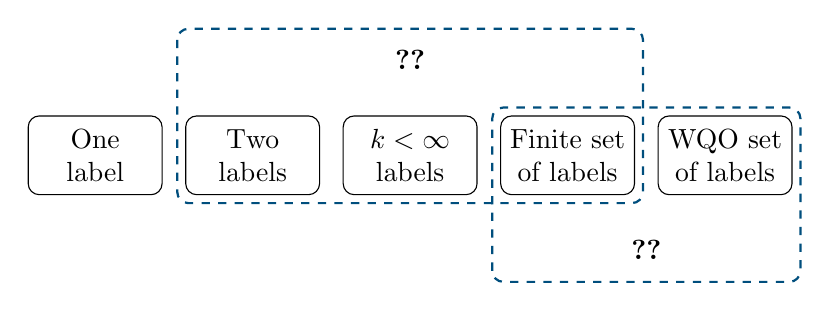
\begin{tikzpicture}[
        conj/.style={rounded corners, thick, dashed, 
            A4
        },
        impl/.style={->, double},
        constr/.style={rounded corners,minimum width=1.7cm,minimum height=1cm,draw,rectangle,align=center}]
        \node[constr] (1w) at (0,0) {One \\ label};
        \node[constr] (2w) at (2,0) {Two \\ labels};
        \node[constr] (kw) at (4,0) {$k < \infty$ \\ labels};
        \node[constr] (lw) at (6,0) {Finite set \\ of labels};
        \node[constr] (ww) at (8,0) {WQO set    \\ of labels};

        \draw[conj]
        ($(lw.south west) + (-0.1, -1.1)$) rectangle ($(ww.north east) + (0.1, 0.1)$);

        \draw[conj]
        ($(2w.north west) + (-0.1, 1.1)$) rectangle ($(lw.south east) + (0.1, -0.1)$);
        \coordinate (P1m) at ($(2w.north)!0.5!(lw.north)$);
        \coordinate (P2m) at ($(lw.south)!0.5!(ww.south)$);
        \node (P1) at ($(P1m) + (0, 0.7)$) {\cref{pouzet1:conj}};
        \node (P2) at ($(P2m) + (0, -0.7)$) {\cref{pouzet2:conj}};

    \end{tikzpicture}
    \caption{The four well-quasi-ordering properties one can consider
             on classes of finite graphs.}
    \label{graph-properties:fig}
\end{figure}

In general, the class of all finite graphs (even undirected and unlabelled) is
not well-quasi-ordered under the induced subgraph relation (for instance, the
class of finite cycles forms an infinite antichain).

There have been many attempts to understand
which classes of (finite) graphs are WQOs when endowed with the induced
subgraph relation. One can think of the early work of Ding on classes of
bounded tree-depth \cite{DING92}, or more recent approaches
\cite{DRT10,DLP17,POZA22}.
Typical proofs that a set is well-quasi-ordered can be clustered into two
categories: \emph{structural proofs} that exhibit an encoding of the set into a
well-quasi-ordered set built from simpler elements, and \emph{minimal bad
sequence arguments} \cite{NASH65}. The latter are often tedious and error-prone
to carry out \cite[Discussion xxx]{LOPEZ23}. 

Attempts to prove these conjectures often relied on assuming some kind of
structural property of the class of graphs, such as enjoying suitable
\emph{tree decompositions}.

Now, to work on those trees, one needs to place a well-quasi-ordered relation
on them. This is usually done using the tree embedding relation, also known as
Kruskal's embedding relation, which is a well-quasi-ordering on trees
\cite{KRU72}. This works when the function that maps a tree to a graph is
simple enough, but more often than not, this is not the case. In \cite{DRT10},
the authors introduce a \emph{tailored} embedding relation on trees, and prove
that it is a well-quasi-ordering under certain hypotheses, leveraging a tedious
and error-prone proof using a \emph{minimal bad sequence argument}
\cite{NASH65}. \todo{talk about clique width now}

We know since \cite{FREU20} and \cite{LOPEZ23} that one can easily inductively
define well-quasi-orderings of increasing complexity on a given set. One
example of such a construction is the \emph{gap embedding relation} of
Derhowitz and Tzameret \cite{DERSHOWITZ200380}. This relation was already at
the core of \emph{priority channel systems}, although in a somewhat hidden form
\cite{HSS13}.  It was also noticed in \cite{LOPEZ24} that the \emph{ad-hoc}
construction of \cite{DRT10} was in fact a particular instance of the gap
embedding relation on trees.

A line of research initiated in \cite{LOPEZ24} explores the \emph{automata
theoretic} approach to the Pouzet conjectures. It was conjectured that the
notion of gap-embedding could be useful. We prove that this is the case.
\todo{Relied on monoids and automata theory on words}
\textbf{The gap embedding is essentially the only well-quasi-ordering on 
graph that can exist.}


Recently, a conjecture was formulated by Sylvain Schmitz in a personal
communication with the authors, which we will call the \emph{transduction
conjecture}. It attemps to bridge the gap between the study of
\kl{well-quasi-ordered} classes of graphs that are ``combinatorially
well-behaved'' and the field of ``structural graph theory'' that focuses on
class that are ``first-order well-behaved''.


\begin{conjecture}[Schmitz's Transduction Conjecture]
    \label{transduction:conj}
    Let $\Cls$ be a class of finite graphs.
    Then, $\Cls$ is labelled-well-quasi-ordered
    if and only if
    $\Cls$
    does not existentially transduce all finite paths.
\end{conjecture}


\paragraph*{Contributions.} At the core of our analysis is the fundamental
connection between a deep automata theoretic construction (the existence of
\emph{forward ramseyan factorisations} on trees \cite{COLC07}) and a deep
combinatorial construction (\emph{gap embedding} on trees
\cite{DERSHOWITZ200380}). These two constructions were meant to be used
together, as we will try to advocate in this paper.

We are also interested in the \emph{decidability} of the WQO property. This is
a question that has recently gained traction in the community, and is of
practical interest.

\begin{theorem}[restate=pouzet2:thm]
    \label{pouzet-2:thm}
    Let $\Cls$ be a class of finite graphs of bounded clique-width.
    Then, $\Cls$ is labelled-well-quasi-ordered
    if and only if 
    $\Cls$ is wqo-well-quasi-ordered.
\end{theorem}

An interpretation is monotone if it is monotone with respect to the
embedding relation.

\begin{theorem}[restate=transductions-paths:thm,label={transductions-paths:thm}]
    \label{transductions-paths:thm}
    Let $\Cls$ be a class of \kl{bounded clique-width}.
    Then $\Cls$ is \kl{labelled-well-quasi-ordered}
    if and only if
    it does not \kl{monotonely transduce}
    all \kl{finite paths}.
\end{theorem}


\begin{conjecture}[Szymon's Collapsing Conjecture]
    \label{nip-cw:conj}
    Let $\Cls$ be a class of graphs.
    If $\Cls$ is labelled-wqo,
    then $\Cls$ is of bounded clique-width.
\end{conjecture}

The motto would then be ``the only well-quasi-orderings on graphs are the gap
embeddings'' and would provide a fundamental barrier to the complexity of
induced subgraph well-quasi-orderings.

\paragraph*{Outline.}

\section{Preliminaries}
\label{sec:preliminaries}

\paragraph*{Automata Theory.} We assume basic familiarity with
automata theoretic concepts such as finite monoids, bottom-up tree automata,
$\MSO$ on trees, and the connection between these three items. We refer to
\textbf{TODO: cite} for a comprehensive introduction to these topics
 \cite{THOM97}.

\paragraph*{Relational Structures.} A \intro{relational signature} is a tuple
$\sigma = (R_1, \ldots, R_k)$ where each $R_i$ is a relation symbol of arity $1
\leq n_i < \omega$. A \kl{(finite) relational structure} over $\sigma$ is a tuple $A
= (U, R_1^A, \ldots, R_k^A)$ where $U$ is a finite set and each $R_i^A
\subseteq U^{n_i}$. We refer to \cite{EBBFLU95} for a comprehensive introduction
to finite model theory.

\begin{itemize}
    \item first order logic 
    \item monadic second order logic
\end{itemize}

\paragraph*{Graphs.} A \intro{graph} is a pair $G = (V, E)$ where $V$ is a set
of \intro{vertices} and $E \subseteq V \times V$ is a set of \intro{edges}. A
graph is \intro{undirected} if $(u, v) \in E$ implies $(v, u) \in E$ for all
$u, v \in V$. In this paper we will focus on finite undirected graphs. Given a
set $X$, an \intro{$X$-labelled graph} is a graph equipped with a function
$\ell \colon V \to X$ that assigns a label to each vertex. Given a class $\Cls$
of finite undirected graphs, write $\Label{X}{\Cls}$ for the class of freely
$X$-labelled graphs in $\Cls$, i.e., the class of all \kl{$X$-labelled graphs}
$G = (V, E, \ell)$ such that $G \in \Cls$.

\paragraph*{Trees.} In this paper, trees are finite, unranked, and unordered.
They are understood as \kl{relational structures} over the \kl{signature}
$\sigma = (\treeleq)$ where $\treeleq$ is the \kl{ancestor relation} and Trees
can be edge-labelled using a finite monoid $M$, where the labelling is
compatible with the transitivity of the ancestor relation.

\AP We use ordered binary trees $T$ with labels taken from a finite alphabet
$\Sigma$ placed on the nodes of the trees. These trees are denoted using
$\Trees{\Sigma}$. In a tree, the root is denoted by $\treeRoot$, and the set of
leaves is denoted by $\Leaves{T}$. Given two nodes $x$ and $y$ in a tree $T$,
their least common ancestor is denoted by $\lca(x,y)$. Given two nodes $x,y$
such that $y$ is an ancestor of $x$, the notation $T[x:y]$ denotes the
\emph{word} in $\Sigma^*$ obtained by reading the labels of the nodes on the
path from $x$ to $y$ in $T$. 

\AP
A \intro{branch} of a tree $T$ is a maximal totally ordered subset of $T$.

\paragraph*{Transductions.} An \intro{$\MSO$-interpretation} between two
classes $X$ and $Y$ of finite relational structures is given by formulii
$\phi_{\Delta}, \phi_{\delta}, \phi_{R}$ in \kl{monadic second-order logic}.
The interpretation defines a relation between structures of $X$ and $Y$ as
follows: ... We define similarly the notion of \intro{existential
transduction}.

\paragraph*{Bounded clique-width.} A class of graph has \intro{bounded
clique-width} if it is included in the image of some \kl{$\MSO$-interpretation}
from finite trees to finite undirected graphs \cite{COUR91}


\paragraph*{Well-quasi-orderings.} A quasi-ordered set $(X, \leq)$ is a set $X$
equipped with a reflexive and transitive relation $\leq$. A sequence
$\seqof{x_i}$ of elements in $X$ is \intro(sequence){good} if there exist $i <
j$ such that $x_i \leq x_j$. A quasi-ordered set is \intro{well-quasi-ordered}
(\reintro{wqo}) if every infinite sequence is \kl(sequence){good}.

\AP Let $(X, \leq)$ be a quasi-order, and let $\Cls$ be a class of
\kl{$X$-labelled graphs}. Then, we define the \intro{$X$-induced quasi-order}
on $\Cls$ as follows: for $G, H \in \Cls$, we write $G \leq H$ if there exists
a \kl{monomorphism} $f \colon G \to H$ such that for all $v \in V$, we have
$\ell_G(v) \leq \ell_H(f(v))$. 

\AP A class $\Cls$ of finite undirected graphs is
\intro{labelled-well-quasi-ordered} (\reintro{labelled-wqo}) if for every
finite set $(X,=)$, the class $\Label{X}{\Cls}$ is \kl{well-quasi-ordered}
using the \kl{$X$-induced quasi-order}. A class of graph is
\intro{wqo-well-quasi-ordered} (\reintro{wqo-wqo}) if for every
\kl{well-quasi-order} $(X, \leq)$, the class $\Label{X}{\Cls}$ is
\kl{well-quasi-ordered} using the \kl{$X$-induced quasi-order}.








%!TEX root = ../cwqo.lipics.tex
\section{From Clique Width to Linear Clique Width}
\label{sec:bad-patterns}




In this section, we will prove the main theorem of this paper, which provides
an effective algorithm to decide if a class of graphs of bounded clique-width
is well-quasi-ordered. 

\begin{theorem}[restate=effective-image:thm,label={effective-image:thm}]
    \label{effective-image:thm}
    Let $I$ be an $\MSO$ interpretation
    from finite trees to undirected graphs.
    There exists a computable $k \in \Nat$
    such that $\image{I}$
    is $k$-well-quasi-ordered
    if and only if 
    $\image{I}$ is wqo-well-quasi-ordered.
    These properties are furthermore decidable.
\end{theorem}

From this theorem, we immediately provide a positive answer to
\cref{pouzet2:conj} for classes of graphs of \kl{bounded clique-width}.

\begin{corollary}
    \label{effective-image:cor}
    A class of graphs $\Cls$ of \kl{bounded clique width} 
    is \kl{labelled-well-quasi-ordered}
    if and only if it is \kl{wqo-well-quasi-ordered}.
\end{corollary}
\begin{proof}
    Consider a class $\Cls$ of graphs having bounded clique width.
    There is an interpretation from trees to a superset of this class $\Cls$.
    Because $\Cls$ is \kl{labelled-well-quasi-ordered}, the class of images
    can be described using finitely many forbidden patterns,
    and we can assume that we do not take subsets.
    As a consequence, we can assume that there exists a $\varphi$
    such that $\Cls \subseteq \varphi(\Trees{\Sigma}) \subseteq \dwset{\Cls}$.
    Now, because $\Cls$ is \kl{labelled-well-quasi-ordered}, we can assume that
    $\dwset{\Cls}$ is \kl{labelled-well-quasi-ordered} as well.
    This proves that $\varphi(\Trees{\Sigma})$ is \kl{labelled-well-quasi-ordered},
    hence \kl{wqo-well-quasi-ordered},
    and as a consequence so is $\Cls$.
\end{proof}

Before proving \cref{effective-image:thm}, let us focus our attention on
\intro{simple interpretations}, i.e., those that are defined solely by a
formula $\varphi_E(x,y)$.
This is not a restriction, as the following lemma
shows.

\begin{lemma}
    \label{simple-interpretation:lem}
    Let $I$ be an $\MSO$ interpretation from finite trees to undirected graphs.
    There exists a (computable) simple interpretation $I'$ such that
    for all $k \geq 1$,
    $\image{I}$ is \kl{$k$-well-quasi-ordered} if and only if
    $\image{I'}$ is \kl{$k$-well-quasi-ordered}.
\end{lemma}
\begin{proof}
\end{proof}

\subsection{From Interpretation to Monoids}

\AP In this section, we will use standard construction from automata theory,
and especially the equivalence between $\MSO$-formulas on trees and bottom-up
deterministic tree-automata. We refer to the book on Tree Automata Techniques
and Applications for a comprehensive overview of this topic \cite{TATA08}. It
follows from standard arguments that to a formula $\varphi(x,y)$ over binary
trees labelled using letters in $\Sigma$ one can associate a monoid $M$ and a
morphism $\mu \colon \Sigma^* \to M$ such that for any tree $T$ and any pair of
leaves $x,y$ in $T$, whether $T \models \varphi(x,y)$ is entirely determined by
the values of $\mu(T[z \colon x])$, $\mu(T[z \colon y])$ and $\mu(T[\treeRoot
\colon z])$ where $z = \lca(x,y)$ is the \kl{ least common ancestor} of $x$ and
$y$.
As a consequence,
one can collect in a subset $P \subseteq M^3$ all the triples $(a,b,c)$ such
that this triple corresponds to a satisfying assignment of the formula
$\varphi(x,y)$.
This is illustrated in \cref{interpretation-to-monoid:fig}. 

\AP In order to simplify notations and better distinguish between the labels of
the nodes (in a finite alphabet $\Sigma$) and their corresponding elements in
the monoid $M$, we will label the \emph{edges} of the trees by the elements of
$M$, having a special treatment for the root of the tree. Given two nodes $x
\treelt[T] y$ in a tree $T$, we will write $\tlbl{T}{x}{y}$ for the product of
the edge labels on the path from $x$ to $y$ in $T$.  Furthermore, we assume for
the rest of the section that the monoid $M$ and the morphism $\mu$ are fixed,
together with the accepting part $P \subseteq M^3$. As a consequence, when we
refer to trees in this subsection, they have nodes labelled by $\Sigma$ and
edges labelled by $M$. Given such a tree $T$, we define $\treeSem{T}$ as the
graph obtained by considering leaves of $T$ as vertices, and placing an edge
between two leaves $x$ and $y$ if and only if $(\tlbl{T}{z}{x}, \tlbl{T}{z}{y},
\tlbl{T}{\treeRoot}{z}) \in P$ where $z = \lca(x,y)$.

\begin{figure}
    \centering
    \begin{tikzpicture}[
        leaf/.style={
            color=Prune
        },
        lca/.style={
            color=A1
        },
        edge/.style={
            color=A2
        },
        root/.style={
            color=Prune
        },
        gedge/.style={
            color=A4
        },
        ]
        \node[root] (root) at (0,1) {$\treeRoot$};
        \node[leaf] (x) at (-1,-1) {$x$};
        \node[leaf] (y) at (1,-1) {$y$};
        \node[lca] (lca) at (0,0) {$\lca(x,y)$};
        \coordinate (tl) at ($(x.south west)+(-0.2,0)$);
        \coordinate (tr) at ($(y.south east)+(0.2,0) $);
        \coordinate (t)  at ($(root.north)+(0, 1)$);
        \draw[edge,->] (root) to node[midway, left]        {$a$}  (lca);
        \draw[edge,->] (lca)  to node[midway, above  left] {$b$} (x);
        \draw[edge,->] (lca)  to node[midway, above right] {$c$} (y);
        \draw (tl) -- (tr) -- (t) -- cycle;

        \node (maps-to) at (3,0) {$\mapsto$};

        \begin{scope}[xshift=4cm]
            \node[leaf] (nx) at (0,0) {$x$};
            \node[leaf] (ny) at (5,0) {$y$};
            \draw[gedge] (nx) to node[midway, above] {$(a,b,c) \in P$?} (ny);
        \end{scope}
    \end{tikzpicture}
    \caption{The interpretation of a tree using a monoid and an accepting part.}
    \label{interpretation-to-monoid:fig}
\end{figure}

The main idea of using monoids to encode the truth value of $\varphi(x,y)$ is
that one can then use a suitable notion of tree embeddings makes the
interpretation from trees to graphs \emph{monotone}.

\begin{definition}
    \label{composition-ordering:def}
    Let $T_1$ and $T_2$ be two trees. 
    A map $h \colon T_1 \to T_2$ is an \intro{compositional tree embedding}
    if it is a \kl{tree embedding} and
    for all pairs of nodes $x \treelt[T_1] y$ in $T_1$, 
    we have $\tlbl{T_1}{x}{y} = \tlbl{T_2}{h(x)}{h(y)}$.
\end{definition}

\begin{lemma}
    \label{composition-ordering:lem}
    Let $T_1$ and $T_2$ be two trees such that
    $h \colon T_1 \to T_2$ is a \kl{compositional tree embedding}.
    Then, $h \colon \treeSem{T_1} \to \treeSem{T_2}$
    is a \kl{labelled graph embedding}.
\end{lemma}
\begin{proof}
\end{proof}

\AP As a consequence, it is sufficient to understand when the \kl{composition
ordering} on trees is well-quasi-ordered to understand when the \kl{labelled
graph embedding} is well-quasi-ordered. Historically, this was (although not
explicitly) the approach taken by \cite{DRT10}. Unfortunately, the composition
ordering on trees is more often than not way more strict than the \kl{induced
subgraph} ordering. It was already observed that the composition ordering on
trees is \kl{well-quasi-ordered} if and only if \emph{for every} $Q \subseteq
M^3$, the class of graphs obtained from trees by considering only the triples
in $Q$ is \kl{labelled-well-quasi-ordered} \cite{LOPEZ24}. To understand what
happens for a precise choice of $Q$, we need to have a finer understanding of
the way trees can be decomposed.




\begin{figure}
    \centering
    \todo[inline]{Draw the composition ordering on trees}
    \caption{The composition ordering on trees}
    \label{composition-ordering:fig}
\end{figure}

\subsection{Forward Ramseyan Splits and Bad Branches}

\def\t{\aTree} \AP The crucial combinatorial ingredient to understand how to
decompose further the trees will come from an adaptation of the classical Simon
Factorisation Theorem for semigroups \cite{SIMO90}, adapted to trees by
Colcombet \cite{COLC07}. A \intro{split of height $N$} of a tree $\t$ is a
mapping $\spt$ from the nodes of $T$ to $\set{1, \dots, N}$. Given a split
$\spt$ and two nodes $x \treelt[\t] y$, we define $\spt(x \colon y)$ to be the
minimal value of $\spt(z)$ for $x \treelt[\t] z \treelt[\t] y$, and $\infty$
otherwise. Two elements $x \treelt[\t] y$ such that $\spt(x) = \spt(y) = k$ are
\intro{$k$-neighbours} if $\spt(x \colon y) \geq k$.

\AP A split $\spt$ is \intro{forward Ramseyan} if for every $k \in \set{1,
\dots, N}$ and every $x, y, x', y'$ in the same class of \kl{$k$-neighbourhood}
with $x \treelt[\t] y$ and $x' \treelt[\t] y'$, we have:
\begin{equation}
    \label{fake-idempotent:eq} 
    \tlbl{\t}{x}{y} = \tlbl{\t}{x}{y} \cdot \tlbl{\t}{x'}{y'} \quad .
\end{equation} 

\AP
In particular, $\tlbl{\t}{x}{y}$ is an \kl{idempotent}, since $\tlbl{\t}{x}{y}
\cdot \tlbl{\t}{x}{y} = \tlbl{\t}{x}{y}$, but $\tlbl{\t}{x}{y}$ and
$\tlbl{\t}{x'}{y'}$ may be different \kl{idempotents}. 

\AP Let us illustrate how one can use \kl{forward Ramseyan splits} to compute
efficiently the value of $\tlbl{\t}{x}{y}$ for any pair of nodes $x \treelt[\t]
y$. We are going to paraphrase the actual content of \cite[Lemma 3]{COLC07},
using the drawing of \cref{fast-computation:fig} to explain the idea. We claim
that to compute the value of $\tlbl{\t}{x}{y}$, one can restrict the
computation to \emph{few} specific segments of the path from $x$ to $y$ with a
\emph{strictly larger} value of $\spt$. The reason is that whenever $x$ and $y$
are separated by many nodes $z$ such that $\spt(z) = \spt(x:y)$, one can
essentially ignore all but the first and last such nodes to speed up
computation. This of course can be applied recursively leading to a fast (and
first-order definable, provided the split $\spt$ is known) algorithm to compute
the value of $\tlbl{\t}{x}{y}$.

\begin{figure}
    \centering
    \begin{tikzpicture}
        \node (s) at (-1,-1) {$\spt \colon $};
        \node (x) at (0,0) {$x$};
        \node (z1) at (2,0) {$z_1$};
        \node (z2) at (4,0) {$z_2$};
        \node (z3) at (6,0) {$\cdots$};
        \node (z4) at (8,0) {$z_3$};
        \node (y) at (10,0) {$y$};

        \node[below of=z1] {$k$};
        \node[below of=z2] {$k$};
        \node[below of=z4] {$k$};
        \node (xz1) at (1,-1) {$> k$};
        \node (z1z2) at (3,-1) {$> k$};
        \node (z4y) at (9,-1) {$> k$};

        \draw (0.2,-0.5) rectangle (9.8,-1.5);
        \draw (1.7,-0.5) -- (1.7, -1.5);
        \draw (2.3,-0.5) -- (2.3, -1.5);

        \draw (3.7,-0.5) -- (3.7, -1.5);
        \draw (4.3,-0.5) -- (4.3, -1.5);

        \draw (7.7,-0.5) -- (7.7, -1.5);
        \draw (8.3,-0.5) -- (8.3, -1.5);


        \draw[->] (x) -- 
        node[midway, above] {$\tlbl{\t}{x}{z_1}$}
        (z1);
        \draw[->] (z1) --
        node[midway, above] {$\tlbl{\t}{z_1}{z_2}$}
        (z2);
        \draw[->] (z2) -- (z3);
        \draw[->] (z3) -- (z4);
        \draw[->] (z4) -- 
        node[midway, above] {$\tlbl{\t}{z_3}{y}$}
        (y);
        \draw[->] (z1) to[bend left=60] 
        node[midway, above] {$\tlbl{\t}{z_1}{z_2} = \tlbl{\t}{z_1}{z_3}$}
        (z4);

    \end{tikzpicture}
    \caption{Fast computation of the value $\tlbl{\t}{x}{y}$
        provided a forward Ramseyan split.}
    \label{fast-computation:fig}
\end{figure}

\AP The main theorem of \cite{COLC07} is that for every finite monoid $M$,
there exists a finite depth $N$ such that for every tree $T$ labelled using
$M$, there exists a forward Ramseyan split of height $N$ for $T$. We can
therefore assume that our trees are always equipped with a forward Ramseyan
split of height $N$.

\AP One can define a notion of embedding between two trees equipped with their
respective \kl{forward Ramseyan splits}. Given two trees $\t_1$ and $\t_2$ with
their respective splits $\spt_1$ and $\spt_2$, a map $h \colon \t_1 \to \t_2$
is a \intro{gap embedding} if it is a \kl{tree embedding} and for all
\kl{$k$-neighbouring} nodes $x \treelt[\t_1] y$ in $\t_1$, $h(x) \treelt[\t_2]
h(y)$ are \kl{$k$-neighbouring} nodes in $\t_2$. Trees equipped with
\kl{forward Ramseyan splits} form a \kl{well-quasi-ordered} set with respect to
the \kl{gap embedding} relation \cite{DERSHOWITZ200380}.

\AP Let us introduce a notion of dependency between nodes that will allow us to
explain how the \kl{gap embedding} relation preserves \emph{some} of the monoid
products in the trees. A node $x$ is \intro{independent at level $k$} from a
node $y$, written $x \bot_k y$ if $x$ is \kl{independent at level $k+1$} and
$\spt(x:y) \geq k+1$ or if there exist three nodes $z_1, z_2, z_3$ such that
$x \treelt[\t] z_1 \treelt[\t] z_2 \treeleq[\t] z_3 \treelt[\t] y$ such that
$\spt(z_1) = \spt(z_2) = \spt(z_3) = k$, $x \bot_{k+1} z_1$, $z_1 \bot_{k+1}
z_2$, and $z_3 \bot_{k+1} y$. If $k = N+1$, then $x \bot_{N+1} y$ if $x$ is the
immediate ancestor of $y$ in the tree.

\begin{lemma}
    Let $h \colon (T, \spt) \to (T', \spt')$ be a \kl{gap embedding} between two
    trees equipped with \kl{forward Ramseyan splits}. Then, for all $x \bot_k y$
    in $T$, we have $\tlbl{T}{x}{y} = \tlbl{T'}{h(x)}{h(y)}$.
\end{lemma}
\begin{proof}
    By immediate induction on $\spt(x:y)$.
\end{proof}

\AP Therefore, the main combinatorial obstacle to understanding whether or not
a class is \kl{labelled-well-quasi-ordered} is to understand the behaviour of
pairs of nodes $x$ and $y$ that are \kl{dependent}. This is the motivation
for the following construction that studies the behaviour of
consecutive \kl{$k$-neighbourhoods} in a tree.

\begin{definition}
    \label{ramseyan-branch:def}
    Let $T$ be a tree and $\spt$ be a \kl{forward Ramseyan split} of height $N$.
    A \intro{bough of level $k$} in $T$ is an infix of a branch of $T$
    satisfying:
    \begin{enumerate}
        \item Its maximal and minimal elements have level $k$
        \item All elements of the bough have level greater or equal to $k$
    \end{enumerate}
    The \intro{size of a bough} is the number of elements of depth $k$
    in the \kl{bough}.
\end{definition}

\AP Let $B$ be a \kl{bough of level $k$} in $T$. Given two nodes $b_1$ and
$b_2$ in $B$ such that $\spt(b_1) = \spt(b_2) = k$, we define the $T_{b_1:b_2}$
as the set of nodes $x$ in $T$ such that $b_1 \treeleq x$ and $\neg (b_2
\treeleq x)$. For every leaf $x \in T_{b_0: b_n}$ where $n$ is the size of the
bough $B$, we define $\Bt(x)$ to be the least ancestor of $x$ that belongs to
$B$. Similarly, we define $\Bl(x)$ to be the least element of $B$ that is
greater or equal to $\Bt(x)$, and $\Br(x)$ to be the greatest element of $B$
that is less or equal to $\Bt(x)$. To every leaf $x$ of $B(T)$, we can
therefore associate a triple of values: $\BtL(x) \defined
\tlbl{\t}{\Bt(x)}{x}$, $\BlL(x) \defined \tlbl{\t}{\Bl(x)}{\Bt(x)}$, and
$\BrL(x) \defined \tlbl{\t}{\Bt(x)}{\Br(x)}$. We refer to
\cref{type-of-a-leaf-in-branch:fig} for an
illustration of the type of a leaf with respect to a given \kl{bough} $B$.
We also refer to \cref{partitionning-a-graph:fig} for an illustration of the
resulting partition of the tree $T$ with respect to a given \kl{bough} $B$.

\begin{figure}
    \centering
    \begin{tikzpicture}[
        branch/.style={
            color=Prune,
            inner sep=0pt,
            minimum size=4pt,
            fill,
            circle
        },
        inner/.style={
            color=A1,
            inner sep=0pt,
            minimum size=4pt,
            draw,
            circle
        },
        staredge/.style={
            color=A1,
            ->,
            dashed
        },
        root/.style={
            color=Prune,
        },
        leaf/.style={
            color=Prune,
        },
        monoid/.style={
            color=A2
        },
        ]
        % first draw the branch 
        \node[root]   (root) at (-2,0) {$\treeRoot$};
        \node[branch] (b0) at (0,0) {};
        \node[branch] (b1) at (4,0) {};
        \node[inner]  (t)  at (2,0) {};
        \node[leaf]   (x)  at (3.5,-2) {$x$};

        \node[above=0.1cm of b0] {$\Bl(x)$};
        \node[above=0.1cm of t]  {$\Bt(x)$};
        \node[above=0.1cm of b1] {$\Br(x)$};

        \draw[staredge] (root) -- (b0);
        \draw[staredge] (b0) -- node[monoid, midway, below] {$\BlL(x)$} (t);
        \draw[staredge] (t)  -- node[monoid, midway, below] {$\BrL(x)$} (b1);
        \draw[staredge] (b1) -- (5,0);

        \draw[staredge] (t)  -- node[monoid, midway, below left] {$\BtL(x)$} (x);
    \end{tikzpicture}
    \caption{The type of a leaf with respect to a given \kl{bough} $B$.}
    \label{type-of-a-leaf-in-branch:fig}
\end{figure}

\begin{figure}
    \centering
    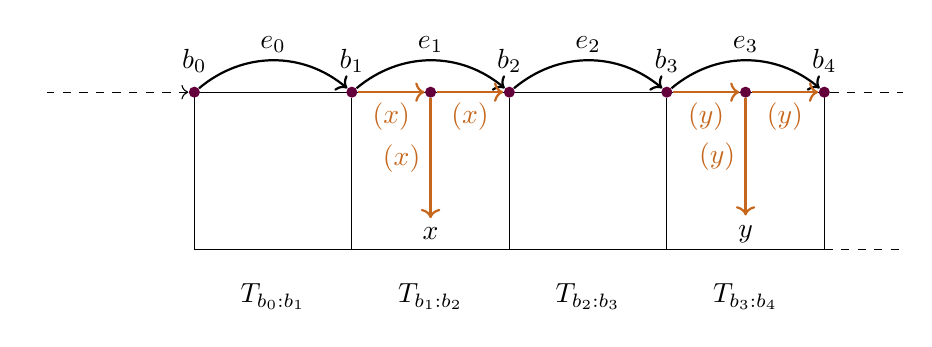
\begin{tikzpicture}[
        localType/.style={
            color=C3,
            thick
        },
        branchProj/.style = {
            color=Prune,
            inner sep=0pt,
            minimum size=4pt,
            fill,
            circle
        },
        leaf/.style={
            color=Prune,
        },
        ]
        \draw (0,0) rectangle (8,2);
        \node (root) at (-2,2) {$\treeRoot$};
        \foreach \x in {0,1,2,3,4} {
            \coordinate (n\x) at ({ 2 * \x},0);
            \coordinate (pb\x) at ({ 2 * \x},2);
            \node[branchProj] (b\x) at (pb\x) {};
            \node (lb\x) at ({ 2 * \x},2.4) {$b_{\x}$};
            \draw (n\x) -- (b\x);
        }
        \draw[dashed,<-] (b0) -- (root);
        \draw[dashed] (b4) -- (9,2);
        \draw[dashed] (n4) -- (9,0);

        \foreach[count=\x] \y in {0,1,2,3} {
            \node (E\x) at ({ 2 * \x - 1},2.6) {$e_{\y}$};
            \draw[->,thick] (b\y) to[bend left=40] (b\x);
            \node (T\x) at ({ 2 * \x - 1},-0.6) {$T_{b_{\y}:b_{\x}}$};
        }
        
        \node (x) at (3,0.2)  {$x$};
        \node (y) at (7,0.2)  {$y$};
        \node[branchProj] (tx) at (3,2) {};
        \node[branchProj] (ty) at (7,2) {};

        \draw[localType, <-] (x)  -- 
        node[midway, left] {$\BtL(x)$} (tx);
        (tx);
        \draw[localType, ->] (tx) -- 
        node[midway, below] {$\BrL(x)$}
        (b2);
        \draw[localType, <-] (tx) -- 
        node[midway, below] {$\BlL(x)$}
        (b1);

        \draw[localType, <-] (y)  -- 
        node[midway, left] {$\BtL(y)$} 
        (ty);
        \draw[localType, ->] (ty) -- 
        node[midway, below] {$\BrL(y)$}
        (b4);
        \draw[localType, <-] (ty) --
        node[midway, below] {$\BlL(y)$}
        (b3);


    \end{tikzpicture}
    \caption{Partitionning a graph using a branch.}
    \label{partitionning-a-graph:fig}
\end{figure}

\AP
To compute the presence of an edge between two leaves $x$ and $y$
in $B(T)$, we only need to know their respective \kl{bough types}
the order in which they appear in the \kl{bough}, 
and whether or not there is an idempotent. \cref{partitionning-a-graph:fig}.

\begin{definition}
    \label{good-bough:def}
    Let $B$ be a \kl{bough} of level $k$ in $T$.
    We say that $B$ is a \intro{good bough} if, for every element $m \in M$,
    there exists a \kl{bough} $H$ of level $k$ in some other tree $T'$,
    and a function $h \colon B(T) \to H(T')$ (from leaves to leaves) such that
    \begin{enumerate}
        \item The subgraph generated by $m B(T)$ 
            is an \kl{induced subgraph} of $H(T')$
            via $h$.
        \item The image of the first block of $B$ by $h$
            is contained in the first block of $H$.
        \item The image of the last block of $B$ by $h$
            is contained in the last block of $H$.
        \item The map $h$ respects the \kl{bough-types} of the leaves.
        \item The map $h$ respects the \kl{idempotent} directly on the left
            and \emph{directly on the right of the leaves}.
        \item There exists a block of $H$ that does not intersect
            the image of $B$ by $h$.
    \end{enumerate}
\end{definition}

\begin{lemma}
    \label{bad-bough-wqo:lem}
    Assume that there are no bounds on the $k$-length of \kl{bad boughs}, then 
    the class of images is not $(3 \times \card{M}^3 + 1)$-well-quasi-ordered.
\end{lemma}
\begin{proof}
    Let $\seqof{B_i}$ be an infinite sequence of bad branches of strictly increasing $k$-length.
    This means that for every $i$ there exists an $m_i \in M$ such that
    no other \kl{bough} $H$ can contain $m B_i(T)$. 
    By extracting a subsequence, we can assume that $m$ is constant.
    Extracting more, we can assume that the $k$-length of $B_i$ is greater than three times the
    number of nodes in $B_{i-1}$.

    Look at the generated graphs, where nodes are labelled by the \kl{bough
    types} of the leaves plus distinguishing colors for the first and last
    elements of the branches if it is defined, and a special color otherwise.
    That is, we have $3 \times \card{M}^3 + 1$ different labels.

    Assume by contradiction that there exists an embedding from $T_i$ to $T_j$
    for some $i < j$. Then, this is also an embedding between $B_i(T_i)$ and
    $B_i(T_j)$, and shows that $B_i(T_i)$ is a \kl{good branch} which is a
    contradiction.
\end{proof}

\AP What \cref{bad-bough-wqo:lem} shows is that the presence of arbitrarily
long ``unbreakable" \kl{boughs} prenvents the class of images from being
\kl{labelled-well-quasi-ordered}. The next step will be to show that provided a
bound on the length of the \kl{bad boughs}, the class of images is
\kl{labelled-well-quasi-ordered}.  To that end, we will 
prove that \kl{good boughs} are in fact easily recognizable
using $\MSO$, hence obtain a decidability result.

\begin{lemma}
    \label{good-bough-recognizable:lem}
    Let $T$ be a tree and let $B$ be a \kl{good bough}.
    Then one can assume that $H$ is three copies of $B$.
\end{lemma}
\begin{proof}
    Let $H$ together with $h$ be a witness that $B$ is a \kl{good bough}.
    Let us define the following embedding $k \colon B \to BBB$.
    For every leaf $x$ in $B$, if $h(x)$ is \emph{before} the untouched graph
    of $H$, then $k(x) = (x,1)$ the first copy of $B$.
    Otherwise, $k(x) = (x,3)$ the third copy of $B$.

    Let us check that $k$ respects the required properties.
    First, $k$ respects the \kl{bough-types} of the leaves by construction.
    Second, $k$ respects the \kl{idempotent} directly on the left and right
    by construction too.
    Third $k$ respects the last block and first-block conditions, because $h$
    did.

    Finally, the only thing left to check is that $(x,y)$ is an edge in the
    graph $B$ if and only if $(k(x), k(y))$ is one in $BBB$.
    If $x$ and $y$ are sent on the same copy, there is nothing to be done.
    If $x$ and $y$ are separated, then
    they were already separated in $H$.
    As a consequence, the presence of an edge between $x$ and $y$ in $B$ is
    equivalent to the presence of an edge between $h(x)$ and $h(y)$,
    but these introduce an idempotent node between them,
    and therefore the same thing holds between $k(x)$ and $k(y)$: indeed,
    the inserted idempotent node \emph{must have the same value}
    because $h$ preserved this!
\end{proof}

As a consequence, checking whether a \kl{bough} is \kl{good} is $\MSO$
definable, one simply has to guess a partition of $B$ into two different
copies.

\begin{lemma}
    \label{bad-boughs-decidable:lem}
    One can decide whether there exists unbounded
    \kl{bad boughs}.
\end{lemma}
\begin{proof}
    We consider the automaton that reads from a decorated tree
    the bough $B$, the partition, the type of the leaves. 
    It first checks that the decoration is correct, and then
    guesses whether the decoration would still be good when
    mapping every leaf of the bough to either a "left" or a "right"
    duplicate of this branch. This is an $\MSO$-definable property.
    It suffices to check that the corresponding automaton
    has an unbounded language, which is decidable.
\end{proof}

\subsection{Good Expansion of A Tree}


In this subsection, we will prove the converse of \cref{bad-bough-wqo:lem},
i.e., we are going to build a suitable embedding provided that the length of
the \kl{bad boughs} is bounded.
To that end, let us first define the \kl{good expansion} of a tree.

\AP Assume that there is a bound $K$ on the length of \kl{bad boughs}, then one
can embed any Ramseyan tree $(T, \spt)$ into a Ramseyan tree $(T',\spt')$ such
that every \kl{$k$-neighbourhood} in $T'$ is \emph{split}. We will therefore
work on trees $(T, \spt, \Delta)$ where $\Delta$ is a subtree of $T$ consisting
of \emph{important nodes}.
We can refine our notion of \kl{gap embedding} to respect important nodes.

\begin{definition}
    The \intro{generalized gap embedding relation}
    between trees.
    It is a map $h \colon T \to T'$ such that
    $h$ is a \kl{gap embedding} between $(T, \spt)$
    and $(T', \spt')$,
    and furthermore if $x \treelt y$ are such that
    $\spt(x) = \spt(y)$ and $\spt(x:y) > k$,
    then $h(x) \treelt h(y)$ are such that
    $\spt'(h(x)) = \spt'(h(y))$ and $\spt'(h(x):h(y)) > k$.
    Furthermore, every node $x$ is labelled 
    with the values of $\tlbl{\t}{z}{x}$ for the first nodes
    $z$ of depth $k$ among ancestors of $x$.
\end{definition}

\begin{lemma}
    If $T$ embeds into $T'$ via the \kl{generalized gap embedding relation}
    then their \kl{marked subgraphs} embed into each other.
\end{lemma}
\begin{proof}
    We prove by induction on $\spt(x:y)$ that
    $\tlbl{\t}{z}{x} = \tlbl{\t'}{h(z)}{h(x)}$ for marked nodes.
    If $\spt(x:y) = \infty$, then the result is immediate.
    If $\spt(x:y) = k$, then
    either $x$ and $y$ are separated by some $z$ that is unmarked
    and the result is immediate, or $x$ and $y$ are only separated by

    \todo[inline]{proof}
\end{proof}


In general, it is not true that the \kl{generalized gap embedding relation}
is a \kl{well-quasi-ordering}. However, we have a bound on the maximal
distance between two marked nodes, and this allows us to prove the following
theorem.

\begin{theorem}
    Let $d$ be a number. The class of all $(T, \spt, \Delta)$
    such that the distance between two marked nodes at level $k$
    is either at most $d$, or they are separated by at least $2$ unmarked nodes
    at level $k$ is \kl{labelled-well-quasi-ordered}.
\end{theorem}

Using this theorem, we conclude this section.

\begin{proofof}{effective-image:thm}[main]
    Test
\end{proofof}


\section{Neighbour Respecting Gap-Embedding}
\label{sec:neighbour-respecting-gap-embedding}

The goal of this subsection is to prove that the gap-embedding relation with a
bounded dependency relation is well-quasi-ordered. Unfortunately, encoding the
dependency inside the usual notion of gap-embedding (the one without
dependencies) is non-trivial. We will instead leverage the recent advances in
inductively defined well-quasi-orderings \cite{FREU20,LOPEZ23}, and the
characterization of the gap-embedding relation as an inductive Kruskal
construction \cite{FREU20} to conclude.

\begin{equation*}
    T_{k+1}^N (X) \defined
    \mu Y. T_{k}^N( \cdots T_k^N(Y) \cdots ) + X
\end{equation*}

And then we use \cite{LOPEZ23} to conclude that it is a WQO + induction 
to prove that it respects the "first-$N$-neighbours".
\begin{theorem}
    \label{good-generalized-gap:thm}
    The gap ordering associated to the ramseyan split of height $XXX$ is a well-quasi-ordering.
\end{theorem}
\begin{proof}
    Trivial. \todo{Not at all!!}
\end{proof}

TODOs:
\begin{itemize}
    \item Define the simon's factorisation theorem for trees.
    \item Check that we can assume that "all products are nice" and not just the ones
        appearing in the decomposition.
    \item Define "branch decompositions" and the "type of nodes" in a branch decomposition.
    \item Define a "bad branch"
    \item Prove that arbitrarily large bad branches violate WQO.
    \item Prove that "good branches" can be embedded into three copies of themselves
    \item Define the "good expansion" of a tree $T$ by expanding all good branches.
    \item Update the tree-decomposition of this good expansion to add \emph{non-sibling}
        idempotent nodes.
    \item Prove that the good expansions of a tree $T$ are well-quasi-ordered using a 
        suitable gap embedding.
    \item Conclude that the class of images is WQO.
\end{itemize}

\begin{lemma}
    \label{gap-embedding-ramseyan:lem}
    Let $(\t, \spt)$ be a tree with a forward Ramseyan split of height $N$,
    and $(\t', \spt')$ be another tree with a forward Ramseyan split of height $N$.
    Let $h \colon \t \to \t'$ be a map such that for every $x,y \in \t$
    we have 
    \begin{itemize}
        \item $h$ maps leaves to leaves. (respects the tree shape)
        \item $h(\lca(x,y)) = \lca(h(x), h(y))$  (respects the tree shape)
        \item $h(\spt(x)) = \spt'(h(x))$ (locally respects splits)
        \item on every branch, for every node $x$ that has a successor 
            $\tlbl{\t}{x}{x+1} = \tlbl{\t'}{h(x)}{h(x)+1}$ (locally respects edges)
        \item $\min\setof{ \spt(z) }{x \treeleq[\t] z \treeleq[\t] y} = \min\setof{ \spt'(z) }{h(x) \treeleq[\t'] z \treeleq[\t'] h(y)}$
            (globally respects nestings)
    \end{itemize}
    Then the embedding $h$ satisfies for all $x,y$ such that
    there exists $x \treeleq[\t] z_1 \treelt[\t] z_2 \treeleq[\t] y$, 
    with $\spt(z_1) = \spt(z_2) = \min\setof{\spt(z)}{x \treeleq[\t] z \treeleq[\t] y}$, we have
    \begin{equation*}
        \tlbl{\t}{x}{y} = \tlbl{\t'}{h(x)}{h(y)} \quad .
    \end{equation*}
\end{lemma}
\begin{proof}
    We prove this by induction on $k = \min\setof{\spt(z)}{x \treeleq[\t] z \treeleq[\t] y}$.
    The base case is when $k = N$.
    In this case, every node on the path from $x$ to $y$ has \kl{split value} $N$.
    In particular, $\tlbl{\t}{x}{y} = \tlbl{\t}{x}{x+1}$. Now, because $h$ locally 
    respects the edges, we have $\tlbl{\t'}{h(x)}{h(x)+1} = \tlbl{\t'}{h(x)}{h(y)}$,
    and we are done.

    Now, assume that the property holds for $k+1$. Let $x,y$ be such that there
    exists $x \treeleq[\t] z_1 \treelt[\t] z_2 \treeleq[\t] y$ with $\spt(z_1)
    = \spt(z_2) = k$. Let us write $z_3$ for the last node on the path from
    $z_2$ to $y$ such that $\spt(z_3) = k$, and assume that between $x$ and
    $z_1$ there is no node with split value $k$, similarly between $z_1$ and
    $z_2$ and  $z_3$ and $y$.

    By induction hypothesis, we know that $\tlbl{\t}{x}{z_1} =
    \tlbl{\t'}{h(z_2)}{h(z_3)}$. Now, we

\end{proof}

\section{Existentially Interpreting Finite Paths}
\label{sec:interpreting-paths}

TODO:
\begin{itemize}
    \item If not WQO, then arbitrarily large bad branches.
    \item Color the nodes of this bad branch using their type (relative to the branch)
    \item Without loss of generality, assume that the branch is super long, and that
        we do not have a lot of different types of nodes inside each bag.
        (uniform bound $K$)
    \item Take a large bad branch, and define 
        $\psi(x,y) \defined E(x,y) \neq E(l(x), r(y))$ where
        $l(x)$ and $r(y)$ respectively "putting to the left" or 
        "putting to the right" of the branch in a (non-existing) "good decomposition".
    \item Witness that $\psi$ defines \emph{almost} a directed path, except
        that it may have back edges due to the non-commutativity of the idempotent node.
    \item If there are no back edges, we just defined a long induced path.
    \item If there were some back edges, there were \emph{a lot of them}.
    \item Define $\phi(x,y)$ if there exists a directed edge $x \to y$
        \textbf{AND} a node $z$ such that $z \to z_1$, $z \to z_2$
        and a path of length at most $2K$ from $z_1$  to $z_2$
        that goes through $x$ and $y$ (in this order).
    \item Prove that $\phi$ defines a directed path.
    \item Take the symmetric version of $\phi$ and conclude.
\end{itemize}




\section{Structural Graph Theory}

There have been recent results in structural graph theory.

\begin{theorem}[{\cite[Theorem 2.6]{DMT24}}]
    \label{monadically-dependent-patterns:thm}
    Let $\Cls$ be a graph class. Then $\Cls$ is \kl{monadically dependent}
    if and only if for every $r \geq 1$ there exists $k \in \Nat$ such that
    $\Cls$ excludes as \kl{induced subgraphs}:
    \begin{itemize}
        \item all flipped star $r$-crossings of order $k$,
        \item all flipped clique $r$-crossings of order $k$,
        \item all flipped half-graph $r$-crossings of order $k$, and
        \item the comparability grid of order $k$.
    \end{itemize}
\end{theorem}

\begin{corollary}
    \label{wqo-mon-independent:cor}
    Let $\Cls$ be a class of graphs that is 
    \kl{labelled-wqo}. 
    Then $\Cls$ is \kl{monadically dependent}.
\end{corollary}

We go beyond and prove the following class inclusions \kl{labelled-wqo} is
included in \kl{monadically existentially-path free} included in
\kl{monadically dependent}.

\section{Concluding Remarks}
\label{sec:conclusion}

We have proven that for all classes of graphs of bounded clique-width, the
\kl{wqo-wqo} and \kl{labelled-wqo} are two equivalent notions. This result is a
first step towards proving this conjecture for arbitrary classes of graphs.



% Include the bibliography
\bibliographystyle{plainurl}
\bibliography{papers.bib}

% If there are any appendices, we include them here.


\end{document}
